\section{渐开线变压器}
\markboth{52. 渐开线变压器}{52. 渐开线变压器}

\noindent
\begin{minipage}[c]{0.57\textwidth}
  \hspace*{2em}普通变压器中，把若干块矽钢片平行地叠置在一起；但是有一种特殊的变压器，却是把矽钢片弯曲起来，一片紧靠一片地像图 52.1 那样裹在一个圆柱上。应该把矽钢片的中心线弯曲成什么曲线，才能使弯曲后的矽钢片一片紧靠一片地裹紧在圆柱上呢？
\end{minipage}\hfill
\begin{minipage}[c]{0.40\textwidth}
  \centering
  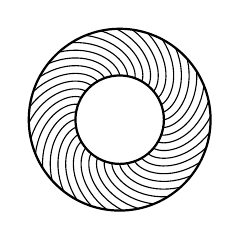
\begin{tikzpicture}[scale=0.78, line cap=round, line join=round]
    \def\r{0.72}
    \def\R{1.48}
    % 渐开线参数 t_max = sqrt((R/r)^2 - 1) = sqrt(3.225) ≈ 1.796
    \pgfmathsetmacro{\tmax}{sqrt((\R/\r)^2 - 1)}

    % 36 片均匀分布的圆渐伸线（矽钢片）
    \foreach \k in {0,10,...,350} {
      \draw[thin, rotate=\k, domain=0:\tmax, samples=22, variable=\t]
        plot ({\r*(cos(\t r) + \t*sin(\t r))},
              {\r*(sin(\t r) - \t*cos(\t r))});
    }

    % 内圆与外圆轮廓
    \draw[thick, fill=white] (0,0) circle (\r);
    \draw[thick] (0,0) circle (\R);
  \end{tikzpicture}
  \captionof*{figure}{图\ 52.1}
\end{minipage}

\medskip

答案是：应该弯曲成圆的渐伸线。

应用工厂里流行的术语来说，就是弯曲成圆的渐开线。正因为如此，这种变压器被取名为渐开线变压器。

为什么要把矽钢片弯曲成圆的渐伸线呢？

为了回答这个问题，我们设圆柱的截面圆半径为 $r$，矽钢片厚度为 $\delta$，并且假定 $\delta$ 比圆柱截面圆的周长 $2\pi r$ 小得多。设总共用 $n$ 片填满圆周，一片厚度为 $\delta$ 的矽钢片占据圆周上长为 $\delta$ 的弧，那么
\[
  n\delta = 2\pi r.
\]
又设矽钢片横截面的面积在弯曲时不变，并且中心线的长度也不变。以上这些假定都是合理的。

如图 52.2，设圆柱的截面圆为圆 $O$，有一片矽钢片的中心线交圆 $O$ 于点 $A$。选取极坐标系，使 $O$ 为极点，$OA$ 为极轴。

\noindent
\begin{minipage}[c]{0.46\textwidth}
  \centering
  \begin{tikzpicture}[scale=0.84, >=Stealth, line cap=round, line join=round]
    \def\r{0.72}
    \def\tmax{1.90}
    \def\halfd{0.055}
    \pgfmathsetmacro{\rhoM}{\r*sqrt(1 + \tmax*\tmax)}
    \pgfmathsetmacro{\angM}{deg(\tmax) - atan(\tmax)}
    \coordinate (O) at (0, 0);
    \coordinate (A) at (\r, 0);
    \coordinate (M) at (\angM:\rhoM);

    % 内外圆
    \draw[thick] (O) circle (\r);
    \draw[thin] (O) circle (\rhoM);

    % 极轴 OA 及其延长与极半径 OM
    \draw[->] (O) -- ({\rhoM+0.35}, 0);
    \draw[->] (O) -- (\angM:{\rhoM+0.38});

    % 矽钢片中心线（渐伸线）及其等距虚线轮廓（厚度 delta）
    \draw[very thick, curveblue, domain=0:2.32, samples=48, variable=\t]
      plot ({\r*(cos(\t r) + \t*sin(\t r))},
            {\r*(sin(\t r) - \t*cos(\t r))});
    \draw[densely dashed, domain=0:2.32, samples=48, variable=\t]
      plot ({\r*(cos(\t r) + \t*sin(\t r)) - \halfd*sin(\t r)},
            {\r*(sin(\t r) - \t*cos(\t r)) + \halfd*cos(\t r)});
    \draw[densely dashed, domain=0:2.32, samples=48, variable=\t]
      plot ({\r*(cos(\t r) + \t*sin(\t r)) + \halfd*sin(\t r)},
            {\r*(sin(\t r) - \t*cos(\t r)) - \halfd*cos(\t r)});

    % 厚度 delta 指示（置于渐伸线最外端，远离 OM）
    \pgfmathsetmacro{\tx}{\r*(cos(2.32 r) + 2.32*sin(2.32 r))}
    \pgfmathsetmacro{\ty}{\r*(sin(2.32 r) - 2.32*cos(2.32 r))}
    \draw[<-, thin] ({\tx - \halfd*sin(2.32 r)}, {\ty + \halfd*cos(2.32 r)})
      -- ({\tx - 0.28*sin(2.32 r)}, {\ty + 0.28*cos(2.32 r)});
    \draw[<-, thin] ({\tx + \halfd*sin(2.32 r)}, {\ty - \halfd*cos(2.32 r)})
      -- ({\tx + 0.28*sin(2.32 r)}, {\ty - 0.28*cos(2.32 r)});
    \node[right=1pt, font=\scriptsize] at ({\tx + 0.24*sin(2.32 r)}, {\ty - 0.24*cos(2.32 r)}) {$\delta$};

    % 角度 theta
    \draw (0.34, 0) arc (0:\angM:0.34);
    \node[font=\scriptsize] at ({\angM/2}:0.49) {$\theta$};

    % 标点与标签
    \fill (O) circle (1.1pt) node[below left=-2pt, font=\scriptsize] {$O$};
    \fill (A) circle (1.1pt) node[below right=-2pt, font=\scriptsize] {$A$};
    \fill (M) circle (1.2pt) node[above right=1pt, font=\scriptsize] {$M(\rho,\theta)$};
    \node[below, font=\scriptsize] at (0.40, 0) {$r$};
    \node[above left=-2pt, font=\scriptsize] at (\angM:{0.56*\rhoM}) {$\rho$};
    \node[below right=-1pt, font=\scriptsize] at ({\r*(cos(1.15 r)+1.15*sin(1.15 r))}, {\r*(sin(1.15 r)-1.15*cos(1.15 r))}) {$s$};
  \end{tikzpicture}
  \captionof*{figure}{图\ 52.2}
\end{minipage}%
\hfill
\begin{minipage}[c]{0.51\textwidth}
\hspace*{2em}设 $M(\rho,\theta)$ 是弯曲矽钢片中心线上任一点，曲线弧 $\arc{AM}$ 的弧长是 $s$。以 $O$ 为圆心、$\rho$ 为半径作圆，与原来半径为 $r$ 的圆围成一个环形，其面积为 $\pi(\rho^2 - r^2)$。一片矽钢片位于这环内的部分，中心线长度为 $s$，厚度为 $\delta$，因而面积为 $s\delta$。环内共有 $n$ 片矽钢片，因而又有
\[
  ns\delta = \pi(\rho^2 - r^2).
\]
\end{minipage}
把 $n\delta = 2\pi r$ 代入，约去 $\pi$ 后得到
\[
  \rho^2 - r^2 = 2rs.
\]
对 $\theta$ 求导，注意 $s' = \sqrt{\rho^2 + \rho'^2}$（第 51 节），得
\[
  2\rho\rho' = 2r\sqrt{\rho^2 + \rho'^2}.
\]
两边除以 $2$，然后平方，得到
\[
  \rho^2\rho'^2 = r^2\rho^2 + r^2\rho'^2,
\]
\[
  \therefore\quad \rho' = \frac{r\rho}{\sqrt{\rho^2 - r^2}}.
\]
由于 $\rho' = \frac{d\rho}{d\theta}$，上式可化为
\[
  \frac{d\theta}{d\rho} = \frac{\sqrt{\rho^2 - r^2}}{r\rho},
\]
式中 $r$ 为常数。积分，得
\[
  \theta = \frac{\sqrt{\rho^2 - r^2}}{r} - \arccos\frac{r}{\rho} + C,
\]
$C$ 为积分常数。由于当 $\rho = r$ 时 $\theta = 0$，得 $C = 0$，因而曲线方程为
\[
  \theta = \frac{\sqrt{\rho^2 - r^2}}{r} - \arccos\frac{r}{\rho}.
\]

下面把曲线方程化成熟知的形式。为此，令
\[
  \varphi = \frac{\sqrt{\rho^2 - r^2}}{r},\quad \alpha = \arccos\frac{r}{\rho},
\]
可得
\[
  \sqrt{\rho^2 - r^2} = r\varphi,\quad \cos\alpha = \frac{r}{\rho},
\]
\[
  \sin\alpha = \sqrt{1 - \left(\frac{r}{\rho}\right)^2} = \frac{\sqrt{\rho^2 - r^2}}{\rho} = \frac{r\varphi}{\rho},
\]
\[
  \theta = \varphi - \alpha.
\]
把极坐标 $(\rho,\theta)$ 化成直角坐标 $(x,y)$，得
\begin{align*}
  x &= \rho\cos\theta = \rho\cos(\varphi - \alpha) \\
    &= \rho(\cos\varphi\cos\alpha + \sin\varphi\sin\alpha) \\
    &= \rho\left(\frac{r}{\rho}\cos\varphi + \frac{r\varphi}{\rho}\sin\varphi\right) \\
    &= r(\cos\varphi + \varphi\sin\varphi), \\
  y &= \rho\sin\theta = \rho\sin(\varphi - \alpha) \\
    &= \rho(\sin\varphi\cos\alpha - \cos\varphi\sin\alpha) \\
    &= \rho\left(\frac{r}{\rho}\sin\varphi - \frac{r\varphi}{\rho}\cos\varphi\right) \\
    &= r(\sin\varphi - \varphi\cos\varphi),
\end{align*}
其中 $r$ 为常数。这正是圆的渐伸线的参数方程（参考第 47 节）。这样就证明了，矽钢片的中心线应该弯曲成圆的渐伸线。
